% ============================================================
%  napkin_first_principles — What should we expect before we simulate?
%  Engine: lualatex   Theme: standard Beamer (Warsaw)
%  All numbers from values/napkin_macros.tex
% ============================================================
\documentclass[aspectratio=169,9pt]{beamer}

\usetheme{Warsaw}
\usecolortheme{default}
\setbeamertemplate{navigation symbols}{}

\usepackage{amsmath,amssymb}
\usepackage{booktabs}
\usepackage{tabularx}
\usepackage{colortbl}

% napkin_macros.tex — AUTO-GENERATED by napkin.py, do not edit

\newcommand{\Napnpvt}{1.580}  % PVT refractive index
\newcommand{\Napthetacdeg}{39.27\,\text{deg}}  % Critical angle: arcsin(1/n)
\newcommand{\NapfTIR}{0.5484}  % TIR fraction (slab): 2cos(θ_c)−1  [Knoll 8.15]
\newcommand{\NapfTIRperend}{0.2742}  % TIR fraction toward one end: f_TIR/2
\newcommand{\Napvgroupmmns}{189.7\,\text{mm/ns}}  % Group velocity: c/n
\newcommand{\NapdEMeV}{2.000\,\text{MeV}}  % Energy deposited: 1-GeV μ⁻ through H=10 mm
\newcommand{\NapRvikuiti}{0.9500}  % Vikuiti non-TIR reflectivity (Materials.cc)
\newcommand{\NapNbounce}{35.00}  % Bounces to traverse L/2 along H-faces
\newcommand{\NapRsurvbounce}{0.1661}  % Vikuiti bounce survival: R^N_bounce
\newcommand{\NapdEdxMeVcm}{2.000\,\text{MeV/cm}}  % MIP dE/dx in PVT (minimum ionising)
\newcommand{\NapLmm}{1400\,\text{mm}}  % Bar length
\newcommand{\NapWmm}{60.00\,\text{mm}}  % Bar width
\newcommand{\NapHmm}{10.00\,\text{mm}}  % Bar height (thin direction)
\newcommand{\Napnsipmperend}{8.000}  % SiPM per END face
\newcommand{\NapyieldejA}{10000\,\text{ph/MeV}}  % EJ-200 scintillation yield
\newcommand{\NaptauriseejA}{0.9000\,\text{ns}}  % EJ-200 rise time
\newcommand{\NaptaudecayejA}{2.100\,\text{ns}}  % EJ-200 decay time
\newcommand{\NaplattmmejA}{3800\,\text{mm}}  % EJ-200 attenuation length (mm)
\newcommand{\NaplattcmejA}{380.0\,\text{cm}}  % EJ-200 attenuation length (cm)
\newcommand{\NapbulksurvejA}{0.8318}  % EJ-200 bulk survival: exp(−700/3800)
\newcommand{\NapNprodejA}{20000\,\text{photons}}  % EJ-200 photons produced: yield×dE
\newcommand{\NapNpesimejA}{1311\,\text{pe}}  % EJ-200 simulated Npe/end at x=0
\newcommand{\NapfeffejA}{0.0655}  % EJ-200 collection×PDE: Npe_sim/N_produced
\newcommand{\NapsigmasimejA}{47.60\,\text{ps}}  % EJ-200 simulated σ(T0) at x=0
\newcommand{\NapsigmaxejA}{6.386\,\text{mm}}  % EJ-200 position resolution: σ·v_g/√2
\newcommand{\NapyieldejB}{10400\,\text{ph/MeV}}  % EJ-204 scintillation yield
\newcommand{\NaptauriseejB}{0.7000\,\text{ns}}  % EJ-204 rise time
\newcommand{\NaptaudecayejB}{1.800\,\text{ns}}  % EJ-204 decay time
\newcommand{\NaplattmmejB}{1600\,\text{mm}}  % EJ-204 attenuation length (mm)
\newcommand{\NaplattcmejB}{160.0\,\text{cm}}  % EJ-204 attenuation length (cm)
\newcommand{\NapbulksurvejB}{0.6456}  % EJ-204 bulk survival: exp(−700/1600)
\newcommand{\NapNprodejB}{20800\,\text{photons}}  % EJ-204 photons produced: yield×dE
\newcommand{\NapNpesimejB}{941.0\,\text{pe}}  % EJ-204 simulated Npe/end at x=0
\newcommand{\NapfeffejB}{0.0452}  % EJ-204 collection×PDE: Npe_sim/N_produced
\newcommand{\NapsigmasimejB}{52.10\,\text{ps}}  % EJ-204 simulated σ(T0) at x=0
\newcommand{\NapsigmaxejB}{6.990\,\text{mm}}  % EJ-204 position resolution: σ·v_g/√2
\newcommand{\NapyieldejC}{9700\,\text{ph/MeV}}  % EJ-230 scintillation yield
\newcommand{\NaptauriseejC}{0.5000\,\text{ns}}  % EJ-230 rise time
\newcommand{\NaptaudecayejC}{1.500\,\text{ns}}  % EJ-230 decay time
\newcommand{\NaplattmmejC}{1200\,\text{mm}}  % EJ-230 attenuation length (mm)
\newcommand{\NaplattcmejC}{120.0\,\text{cm}}  % EJ-230 attenuation length (cm)
\newcommand{\NapbulksurvejC}{0.5580}  % EJ-230 bulk survival: exp(−700/1200)
\newcommand{\NapNprodejC}{19400\,\text{photons}}  % EJ-230 photons produced: yield×dE
\newcommand{\NapNpesimejC}{701.3\,\text{pe}}  % EJ-230 simulated Npe/end at x=0
\newcommand{\NapfeffejC}{0.0361}  % EJ-230 collection×PDE: Npe_sim/N_produced
\newcommand{\NapsigmasimejC}{49.60\,\text{ps}}  % EJ-230 simulated σ(T0) at x=0
\newcommand{\NapsigmaxejC}{6.655\,\text{mm}}  % EJ-230 position resolution: σ·v_g/√2
\newcommand{\NapratiopredejB}{0.8073}  % EJ-204/EJ-200 Npe ratio (napkin prediction)
\newcommand{\NapratioobsejB}{0.7179}  % EJ-204/EJ-200 Npe ratio (simulation)
\newcommand{\NapratiopredejC}{0.6508}  % EJ-230/EJ-200 Npe ratio (napkin prediction)
\newcommand{\NapratioobsejC}{0.5350}  % EJ-230/EJ-200 Npe ratio (simulation)
\newcommand{\Napveffendmmns}{184.6\,\text{mm/ns}}  % Effective propagation velocity (END, EJ-230)
\newcommand{\NapsigmaDtendps}{111.5\,\text{ps}}  % σ of (t_R−t_L) for END estimator
\newcommand{\Napsigmaxendmm}{10.29\,\text{mm}}  % Position resolution: (veff/2)·σΔt
\newcommand{\Napbetaeffenddeg}{13.37\,\text{deg}}  % Effective axial angle END: arccos(veff/vg)
\newcommand{\Napalphacdeg}{50.73\,\text{deg}}  % Angle from bar surface for ray just outside TIR
\newcommand{\Naptanalphac}{1.223}  % tan(α_c) for bounce counting formula
\newcommand{\NapNbounceH}{85.63}  % Bounces on H=10 mm face to reach L/2
\newcommand{\NapNbounceW}{14.27}  % Bounces on W=60 mm face to reach L/2
\newcommand{\NapRviknap}{0.9800}  % Vikuiti reflectivity (napkin, manufacturer spec)
\newcommand{\NapLambdareflHmm}{404.6\,\text{mm}}  % Reflector attenuation length, H=10 mm face
\newcommand{\NapLambdareflWmm}{2428\,\text{mm}}  % Reflector attenuation length, W=60 mm face
\newcommand{\Napsipmactivemmsq}{288.0\,\text{mm2}}  % Total SiPM active area per END face (8×36)
\newcommand{\Napendfacemmsq}{600.0\,\text{mm2}}  % END face area: W×H = 60×10
\newcommand{\Napfcoverage}{0.4800}  % SiPM coverage fraction: 288/600
\newcommand{\NapPDEnapkin}{0.4000}  % Assumed PDE for napkin budget
\newcommand{\NapNtirendC}{5320\,\text{photons}}  % EJ-230: TIR-guided toward one end
\newcommand{\NapNbulksurvC}{2969\,\text{photons}}  % EJ-230: after bulk attenuation (70 cm)
\newcommand{\NapNatsipmC}{1425\,\text{photons}}  % EJ-230: reaching SiPM surface
\newcommand{\NapNpenapkinC}{570.0\,\text{pe}}  % EJ-230: napkin Npe/end (TIR-only path)
\newcommand{\NapNpeLRC}{1140\,\text{pe}}  % EJ-230: napkin Npe L+R total
\newcommand{\Napfescapecone}{0.1129}  % Escape cone fraction at END: (1−cosθ_c)/2
\newcommand{\Napnpeidxmatch}{570.0\,\text{pe}}  % EJ-230 napkin Npe/end (index-matched coupling)
\newcommand{\Napnpeairgap}{234.6\,\text{pe}}  % EJ-230 napkin Npe/end (air-gap escape cone only)
\newcommand{\NapratiovikTIRhi}{2.429}  % Napkin max Vikuiti/TIR ratio (air-gap case ≈ 2.4)
\newcommand{\NapsigmaENDbestps}{53.68\,\text{ps}}  % Best σ_END (m*=8): EJ-230 + Vikuiti, x=0
\newcommand{\NapsigmaTOPbestps}{15.20\,\text{ps}}  % Best σ_TOP (k*=3): EJ-230 + 20 TOP SiPMs
\newcommand{\NapsigmaBLUEbestps}{15.21\,\text{ps}}  % Best σ_BLUE: BLUE combination at x=0
\newcommand{\NapwTOPbest}{0.9870}  % BLUE weight for TOP estimator
\newcommand{\NapwENDbest}{0.0130}  % BLUE weight for END estimator


% ── compact footer ───────────────────────────────────────────
\setbeamertemplate{footline}{%
  \leavevmode\hbox{%
  \begin{beamercolorbox}[wd=0.75\paperwidth,ht=1.8ex,dp=0.8ex,leftskip=3mm]{author in head/foot}%
    \tiny SHiP Timing Bar · First principles before Geant4%
  \end{beamercolorbox}%
  \begin{beamercolorbox}[wd=0.25\paperwidth,ht=1.8ex,dp=0.8ex,rightskip=3mm,right]{date in head/foot}%
    \tiny\insertframenumber%
  \end{beamercolorbox}}}

% ── physics shorthands ────────────────────────────────────────
\newcommand{\thetac}{\theta_c}
\newcommand{\fTIR}{f_{\mathrm{TIR}}}
\newcommand{\latt}{\lambda_{\mathrm{att}}}
\newcommand{\vtg}{v_g}
\newcommand{\veff}{v_{\mathrm{eff}}}
\newcommand{\sigT}{\sigma(T_0)}
\newcommand{\sE}{\sigma_{\mathrm{END}}}
\newcommand{\sT}{\sigma_{\mathrm{TOP}}}
\newcommand{\sB}{\sigma_{\mathrm{BLUE}}}
\newcommand{\Lrefl}{\Lambda_{\mathrm{refl}}}

% ── row highlight ─────────────────────────────────────────────
\definecolor{rowhl}{rgb}{1.0,0.95,0.75}

% ═══════════════════════════════════════════════════════════════
\begin{document}
% ═══════════════════════════════════════════════════════════════

%% ── FRAME 1: TITLE ────────────────────────────────────────────
\begin{frame}[plain]
  \vspace{1.2cm}
  \begin{center}
    {\Large\bfseries What should we expect before we simulate?}\\[6pt]
    {\small First-principles photon budget of a 1.4\,m scintillator bar\\
    for the SHiP Timing Detector}
  \end{center}
  \vspace{0.6cm}
  \begin{center}
    René Ríos \quad·\quad Universidad de La Serena \quad·\quad August 2026
  \end{center}
  \vspace{0.4cm}
  \begin{block}{Central idea}
    {\small Geometry + Snell + exponential attenuation predict the dominant trends
    before any Geant4 output is shown.
    If simulation and napkin disagree, one of them is wrong — finding out which
    is the actual result.}
  \end{block}
\end{frame}

%% ── FRAME 2: THE OBJECT ───────────────────────────────────────
\begin{frame}{The object: one bar of a 50\,m$^2$ detector}
  \begin{columns}[T]
    \column{0.52\textwidth}
      {\small Bar geometry: \NapLmm\ $\times$ \NapWmm\ $\times$ \NapHmm}\\[4pt]
      \begin{itemize}\setlength\itemsep{3pt}
        \item[$\bullet$] 8 SiPMs per END face
        \item[$\bullet$] Up to 70 SiPMs along TOP face
        \item[$\bullet$] $\sim$600 bars for 50\,m$^2$
      \end{itemize}
      \vspace{6pt}
      \begin{block}{Best result tested so far}
        {\footnotesize EJ-230 + END + TOP (20 SiPMs) + Vikuiti:\\
        $\sE=\NapsigmaENDbestps$,\;
        $\sT=\NapsigmaTOPbestps$,\;
        $\sB=\NapsigmaBLUEbestps$\\
        at $x=0$, no electronic jitter.}
      \end{block}

    \column{0.46\textwidth}
      \begin{alertblock}{Optimisation is still open}
        {\footnotesize The best tested point is not proven to be the optimum.
        The question is the Pareto front of $\sigT$ vs.\ number of channels,
        with SiPM jitter and front-end jitter included.}
      \end{alertblock}
  \end{columns}
\end{frame}

%% ── FRAME 3: PHILOSOPHY ──────────────────────────────────────
\begin{frame}{Napkin first — Geant4 second}
  \begin{columns}[T]
    \column{0.48\textwidth}
      \begin{block}{1 — Napkin}
        {\small Snell, geometry and exponential attenuation fix
        the order of magnitude and the \emph{direction} of every trend:
        which material gives more light, which gives better timing.}
      \end{block}

    \column{0.48\textwidth}
      \begin{block}{2 — Geant4}
        {\small Confirms the scale, adds distributions the napkin cannot produce:
        Landau fluctuations, path-length dispersion, angular mixing.}
      \end{block}
  \end{columns}
  \vspace{6pt}
  \begin{alertblock}{}
    {\small\itshape Knoll on optical Monte Carlo: these codes are accurate only to the
    extent that surface reflection, bulk absorption and refractive indices are correct.
    Those are exactly the inputs a napkin calculation can police.}
  \end{alertblock}
\end{frame}

%% ── FRAME 4: STEP 1 — ENERGY DEPOSITION ─────────────────────
\begin{frame}{Step 1 — Energy deposition}
  \begin{columns}[T]
    \column{0.50\textwidth}
      \begin{block}{Bethe–Bloch minimum, through $H = \NapHmm$}
        \[
          \frac{dE}{dx}\approx\NapdEdxMeVcm
          \;\Rightarrow\;
          E_{\mathrm{dep}}\approx\NapdEMeV
        \]
      \end{block}
      \begin{itemize}\setlength\itemsep{3pt}
        \item Sets the scale of everything downstream
        \item Every later factor multiplies this \NapdEMeV
        \item Width is Landau — simulation territory
      \end{itemize}

    \column{0.48\textwidth}
      \begin{alertblock}{What the napkin cannot give}
        {\small Event-by-event Landau fluctuations, $\delta$-ray production,
        path-length variation.  The mean survives; the width is for Geant4.}
      \end{alertblock}
  \end{columns}
\end{frame}

%% ── FRAME 5: STEP 2 — SCINTILLATION YIELD ───────────────────
\begin{frame}{Step 2 — Scintillation yield}
  \begin{columns}[T]
    \column{0.50\textwidth}
      \[N_\gamma = E_{\mathrm{dep}}\cdot Y \approx 2\times 9700 \approx 1.9\times10^4\]
      {\small Optical properties used in simulations:}\\[4pt]
      {\footnotesize
      \setlength{\tabcolsep}{5pt}
      \begin{tabular}{@{}lccc@{}}
        \toprule
        Material & Yield [ph/MeV] & $\tau_d$ [ns] & $\latt$ [cm]\\
        \midrule
        EJ-200 & 10000 & 2.1 & 380\\
        EJ-204 & 10400 & 1.8 & 160\\
        EJ-230 & 9700  & 1.5 & 120\\
        \bottomrule
      \end{tabular}}

    \column{0.48\textwidth}
      \begin{block}{The trade-off}
        {\small Yields agree to within 7\,\%.  What separates the materials
        is how much survives 70\,cm travel ($\latt$) and how fast
        the emission decays ($\tau_d$) — and those two pull in opposite directions.}
      \end{block}
  \end{columns}
\end{frame}

%% ── FRAME 6: STEP 3 — TIR ────────────────────────────────────
\begin{frame}{Step 3 — Total internal reflection}
  \begin{columns}[T]
    \column{0.50\textwidth}
      \begin{block}{Critical angle}
        \[
          \thetac = \arcsin(1/n) = \Napthetacdeg,
          \quad n=\Napnpvt
        \]
      \end{block}
      \begin{block}{Trapped fraction — slab (Knoll Eq.\,8.15)}
        \[
          a = \cos\thetac = 0.774,\quad
          \fTIR = 2a - 1 = \NapfTIR
        \]
        Both walls: $\fTIR/\text{end} = \NapfTIRperend$
      \end{block}

    \column{0.48\textwidth}
      \begin{alertblock}{The bar is not a slab}
        {\small Two wall families must hold TIR simultaneously.
        Knoll Eq.\,8.14 (cylinder, meridional rays) gives $18.4\%$
        per direction — different geometry.}
      \end{alertblock}
      \begin{block}{Key number}
        {\small $\approx\NapfTIRperend$ of photons are guided toward each end.}
      \end{block}
  \end{columns}
\end{frame}

%% ── FRAME 7: STEP 4 — VELOCITY ───────────────────────────────
\begin{frame}{Step 4 — Photon propagation velocity}
  \begin{columns}[T]
    \column{0.50\textwidth}
      \begin{block}{Group velocity}
        \[\vtg = c/n \approx \Napvgroupmmns\]
      \end{block}
      \begin{block}{Effective velocity (END, from Geant4)}
        \[\veff = \Napveffendmmns \;\Rightarrow\; \beta_{\mathrm{eff}}\approx\Napbetaeffenddeg\]
      \end{block}
      {\small$\beta_{\mathrm{eff}}$ is the effective axial angle of the
      photon population that dominates the earliest arrival times.}

    \column{0.48\textwidth}
      \begin{block}{END vs.\ TOP select different photons}
        {\small END is dominated by nearly axial, early photons.
        TOP integrates markedly more diagonal trajectories
        ($\beta_{\mathrm{eff,TOP}}\approx 40^\circ$).
        These two faces carry different timing information.}
      \end{block}
  \end{columns}
\end{frame}

%% ── FRAME 8: STEP 5 — BOUNCES ────────────────────────────────
\begin{frame}{Step 5 — Number of reflections}
  \begin{columns}[T]
    \column{0.50\textwidth}
      \begin{block}{Geometric estimate, ray just outside TIR}
        \[
          N_{\mathrm{bounce}} \approx \frac{d\,\tan\alpha_c}{D},
          \quad \alpha_c = \Napalphacdeg
        \]
      \end{block}
      {\small With $d = 700$\,mm, $\tan\alpha_c = \Naptanalphac$:}
      \vspace{4pt}
      \begin{center}
      {\footnotesize
      \begin{tabular}{@{}lcc@{}}
        \toprule
        Face & $D$ & $N_{\mathrm{bounce}}$\\
        \midrule
        thin ($H$) & \NapHmm & $\approx 86$\\
        wide ($W$) & \NapWmm & $\approx 14$\\
        \bottomrule
      \end{tabular}}
      \end{center}

    \column{0.48\textwidth}
      \begin{alertblock}{Factor of 6 difference}
        {\small The same photon direction produces $\sim$6$\times$ more bounces
        against the 10\,mm face than the 60\,mm face.
        Reflector quality matters more for the thin faces.}
      \end{alertblock}
  \end{columns}
\end{frame}

%% ── FRAME 9: STEP 6 — REFLECTOR LOSSES ──────────────────────
\begin{frame}{Step 6 — Reflector losses become exponential attenuation}
  \begin{columns}[T]
    \column{0.50\textwidth}
      \begin{block}{Survival after $N$ bounces}
        \[P_R = R^N = e^{N\ln R}\]
        \[\Lrefl = \frac{-D}{\tan\alpha_c\cdot\ln R}\]
      \end{block}
      {\small With $R = 0.98$ (Vikuiti, napkin):}
      \vspace{4pt}
      \begin{center}
      {\footnotesize
      \begin{tabular}{@{}lcc@{}}
        \toprule
        Face & $D$ & $\Lrefl$\\
        \midrule
        thin ($H$) & \NapHmm & $\approx 0.4$\,m\\
        wide ($W$) & \NapWmm & $\approx 2.4$\,m\\
        \bottomrule
      \end{tabular}}
      \end{center}

    \column{0.48\textwidth}
      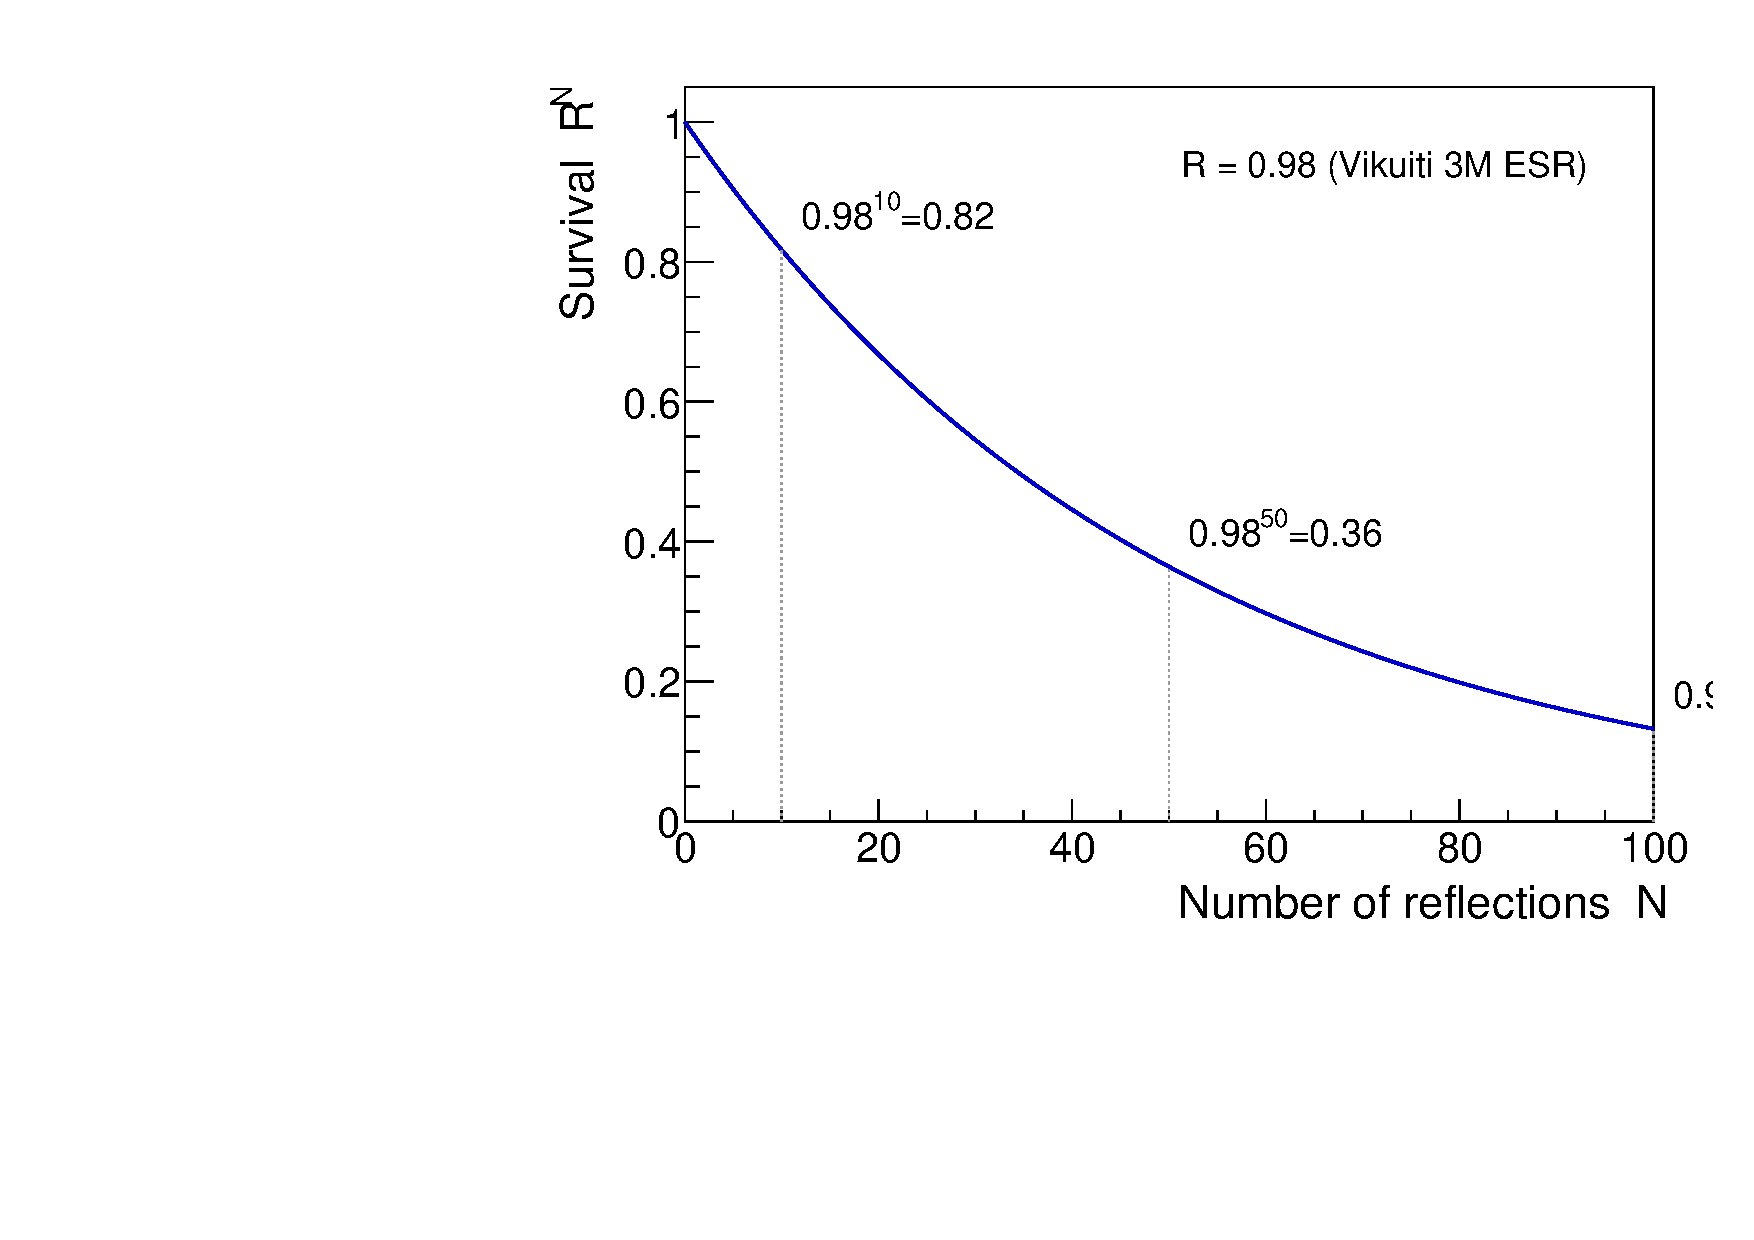
\includegraphics[width=\textwidth,keepaspectratio]{../figs/fig_survival_RN.pdf}
  \end{columns}
\end{frame}

%% ── FRAME 10: STEP 7 — MATERIAL CHOICE ──────────────────────
\begin{frame}{Step 7 — Bulk attenuation and decay time pull in opposite directions}
  \begin{columns}[T]
    \column{0.50\textwidth}
      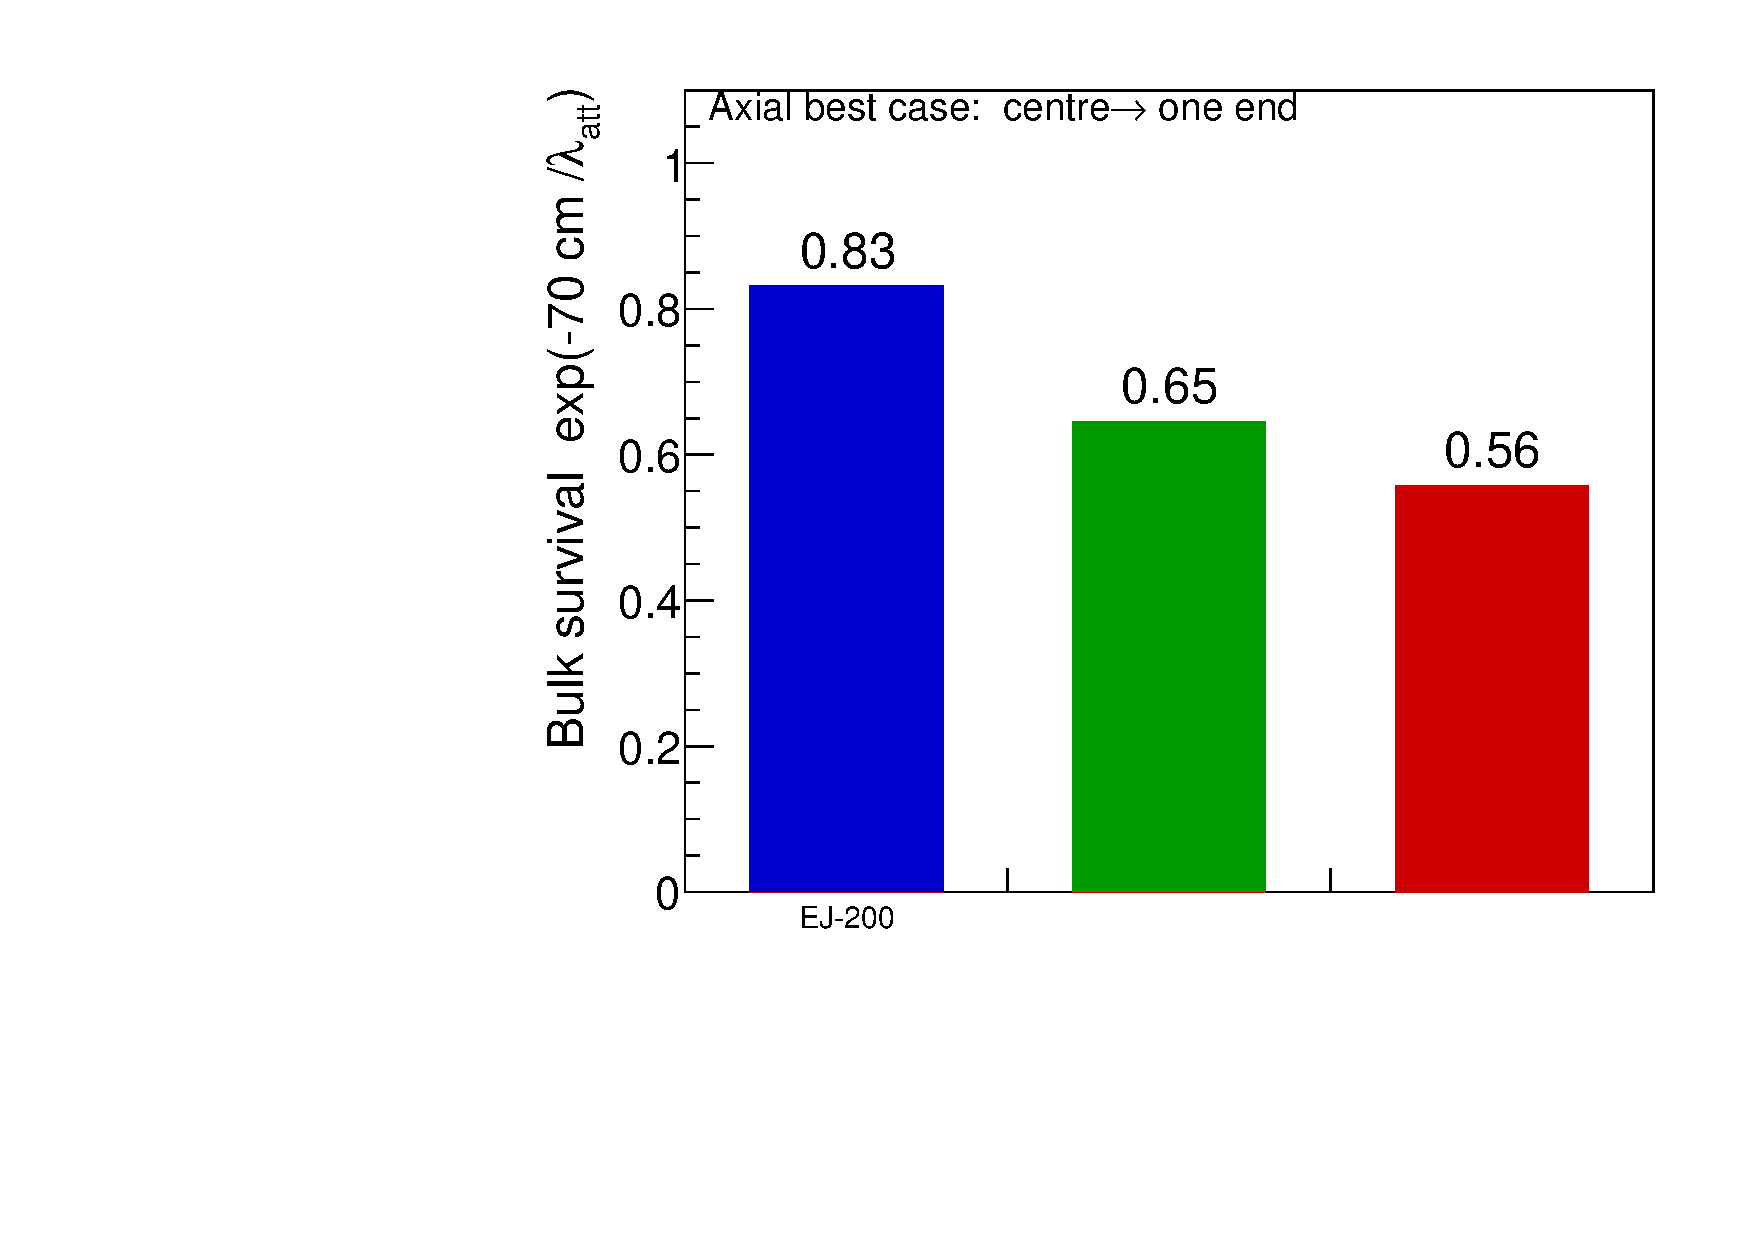
\includegraphics[width=\textwidth,keepaspectratio]{../figs/fig_bulk_survival.pdf}

    \column{0.48\textwidth}
      \begin{block}{Napkin prediction (before the run)}
        {\small EJ-200 delivers the most light (largest $\latt$).\\
        EJ-230 loses the most, but its faster kinetics
        ($\tau_d = \NaptaudecayejC$ vs.\ $\NaptaudecayejA$)
        should win on timing.}
      \end{block}
      \begin{alertblock}{Geant4 confirms both orderings}
        {\small $N_{pe}$: EJ-200 $>$ EJ-204 $>$ EJ-230\\
        $\sigT$: EJ-230 $<$ EJ-204 $<$ EJ-200\\[2pt]
        Both directions as predicted.}
      \end{alertblock}
  \end{columns}
\end{frame}

%% ── FRAME 11: PREDICTIVE VALIDATION ─────────────────────────
\begin{frame}{The ordering was predicted, then observed}
  \begin{columns}[T]
    \column{0.50\textwidth}
      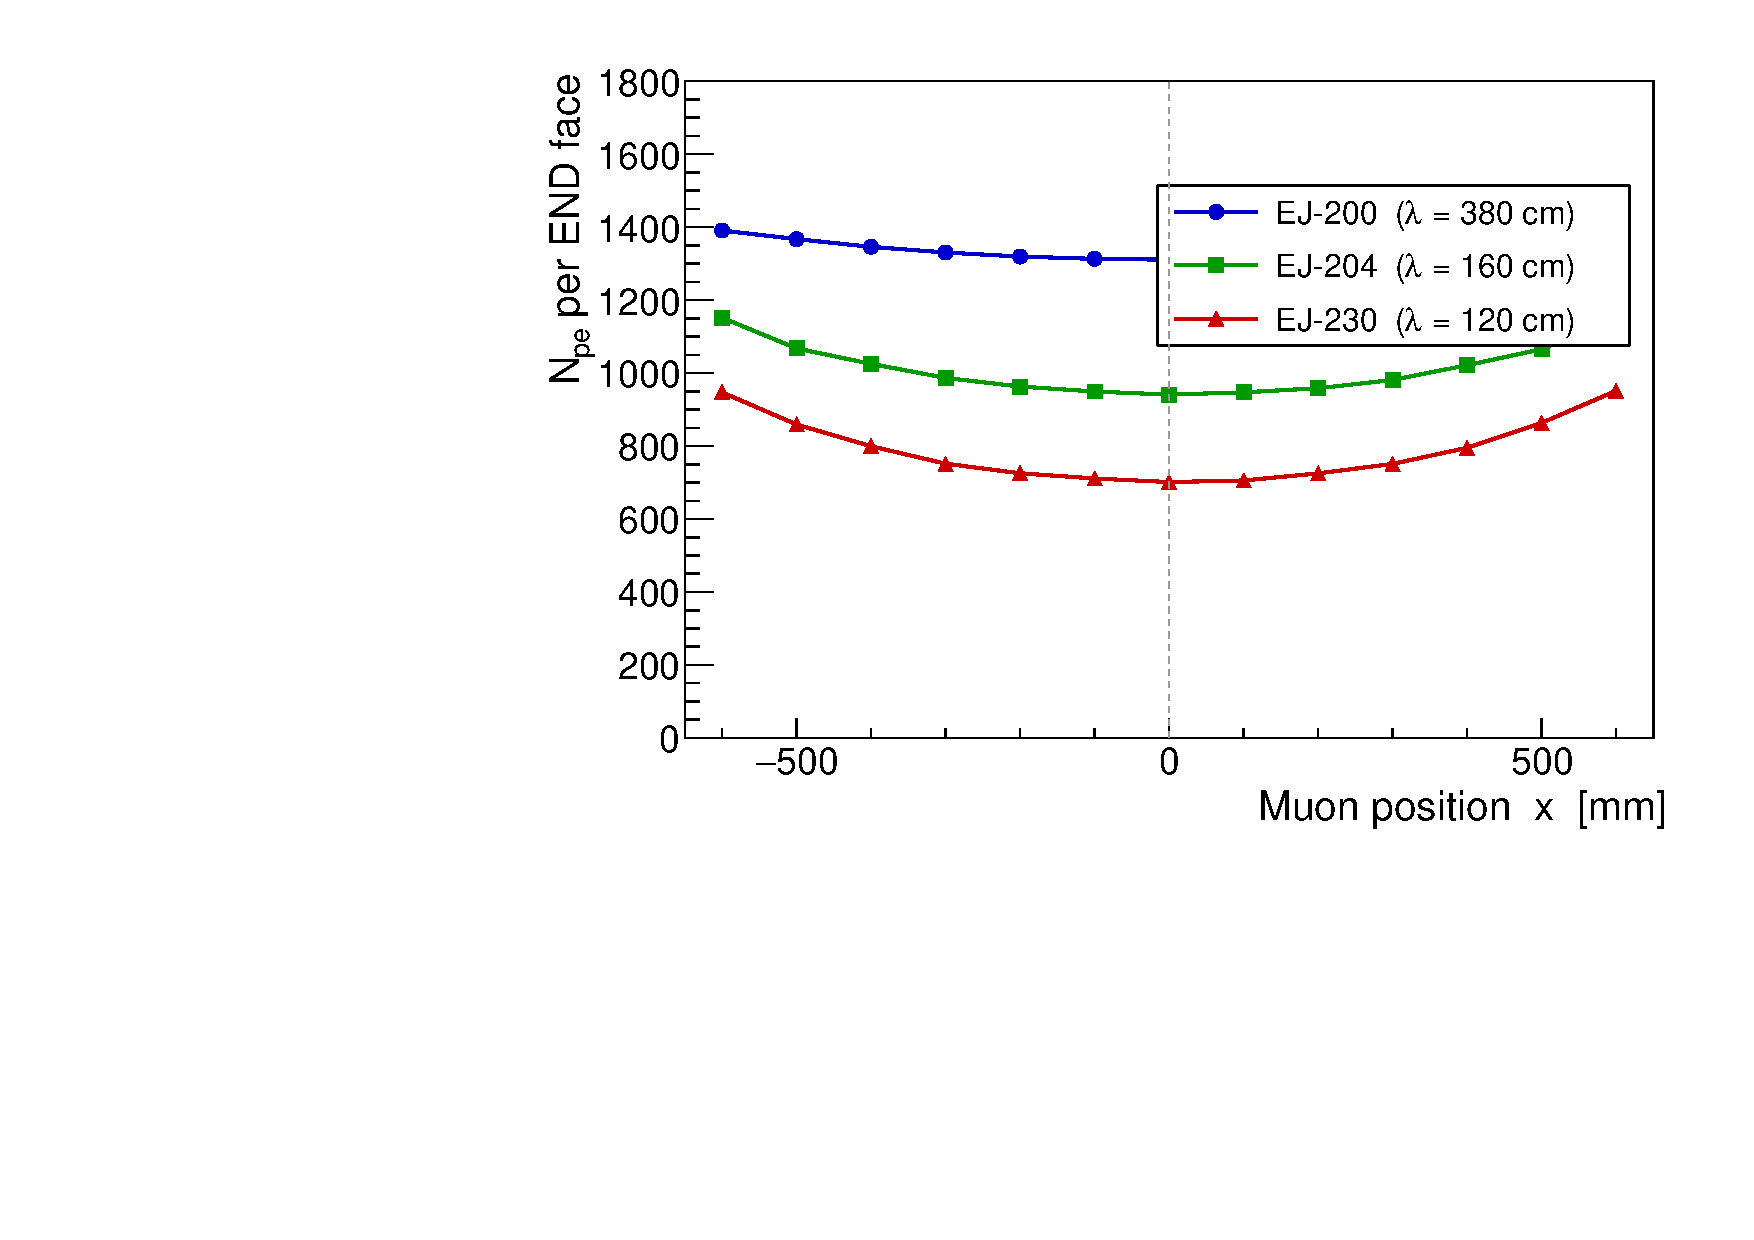
\includegraphics[width=\textwidth,keepaspectratio]{../figs/fig_npe_x.pdf}
      {\tiny $N_{pe}$ per END vs.\ position.  EJ-200 $>$ EJ-204 $>$ EJ-230,
      steeper fall for shorter $\latt$.}

    \column{0.50\textwidth}
      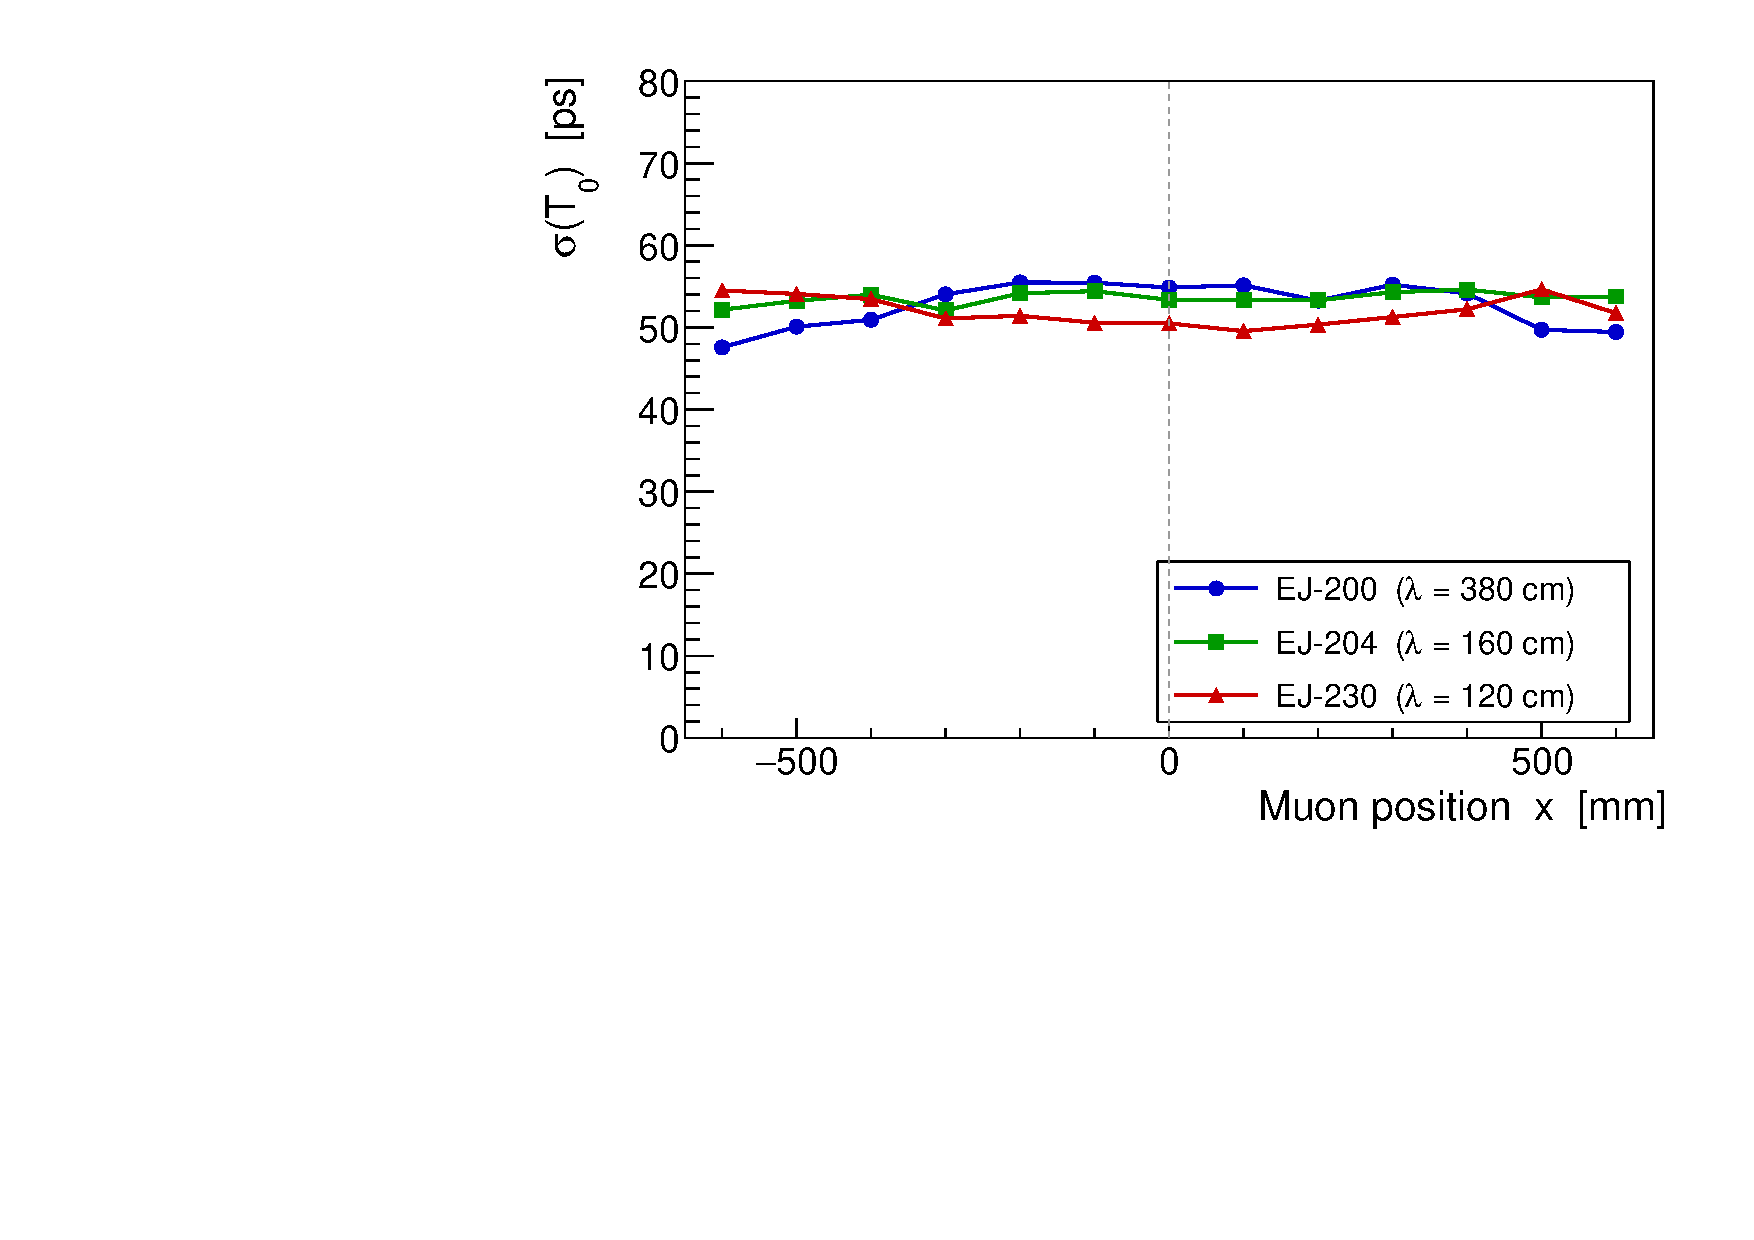
\includegraphics[width=\textwidth,keepaspectratio]{../figs/fig_sigma_t_x.pdf}
      {\tiny $\sigT$ per END vs.\ position.  Ordering inverted: EJ-230 $<$ EJ-204 $<$ EJ-200,
      driven by $\tau_d$.}
  \end{columns}
  \vspace{4pt}
  {\small\itshape
    Two figures, two orderings, opposite directions — written down before the simulation ran.}
\end{frame}

%% ── FRAME 12: PHOTON BUDGET ──────────────────────────────────
\begin{frame}{Closing the chain: photon budget for EJ-230 at $x=0$}
  \begin{center}
  {\footnotesize
  \begin{tabular}{@{}lcc@{}}
    \toprule
    Step & Factor & Cumulative photons\\
    \midrule
    Produced & $Y \times E_{\mathrm{dep}} = 9700\times 2$ & $\sim 1.94\times10^4$\\
    TIR-guided toward one end & $\times\NapfTIRperend$ & $\sim 5300$\\
    Bulk survival (70\,cm) & $\times\NapbulksurvejC$ & $\sim 2970$\\
    End-face coverage (288/600) & $\times\Napfcoverage$ & $\sim 1430$\\
    PDE ($\approx\NapPDEnapkin$) & $\times\NapPDEnapkin$ & $\sim\NapNpenapkinC$\\
    \midrule
    \rowcolor{rowhl}
    Geant4 (EJ-230, END, Vikuiti, $x=0$) & — & $\approx 1400$\,PE\\
    \bottomrule
  \end{tabular}}
  \end{center}
  \vspace{4pt}
  \begin{columns}[T]
    \column{0.50\textwidth}
      \begin{block}{Scale check, not a prediction}
        {\small The chain closes to within 20\,\%.
        The excess is from the reflector-recovered population.
        Factors are not strictly independent.}
      \end{block}
    \column{0.48\textwidth}
      \begin{alertblock}{Count per end — always}
        {\small Mixing a both-ends fraction with a one-end coverage
        silently doubles the answer.}
      \end{alertblock}
  \end{columns}
\end{frame}

%% ── FRAME 13: AUDIT ──────────────────────────────────────────
\begin{frame}{Auditing the 1\,PE anomaly}
  \begin{center}
  {\footnotesize
  \setlength{\tabcolsep}{4pt}
  \begin{tabular}{@{}p{3.5cm}p{3.4cm}p{2.0cm}p{2.0cm}@{}}
    \toprule
    Readout coupling & Acceptance toward one end & PE/end & Vik/TIR ratio\\
    \midrule
    Index-matched & $\NapfTIRperend$ (TIR-guided) & $\approx\Napnpeidxmatch$ & $\approx 1.2$\\
    Air gap (escape cone) & $\Napfescapecone$ & $\approx\Napnpeairgap$ & $\approx 3$\\
    \rowcolor{rowhl}
    \textbf{Reported run} & — & $\approx\mathbf{1}$\,PE & $\approx 10^3$\\
    \bottomrule
  \end{tabular}}
  \end{center}
  \vspace{4pt}
  \begin{columns}[T]
    \column{0.50\textwidth}
      \begin{block}{Escape cone cannot explain $10^3$}
        {\small The cone cuts both Vikuiti and TIR configurations by
        the same factor at the readout face — it cannot generate a ratio.
        The napkin brackets the genuine ratio between 1 and 3.}
      \end{block}
    \column{0.48\textwidth}
      \begin{alertblock}{Falsifiable prediction}
        {\small Run END + TIR-only and END + Vikuiti under identical conditions.
        A ratio near $10^3$ is a surface or RINDEX definition to be found,
        not a physics result.}
      \end{alertblock}
  \end{columns}
\end{frame}

%% ── FRAME 14: OBSERVABLES ────────────────────────────────────
\begin{frame}{From arrival times to physical observables}
  \begin{columns}[T]
    \column{0.52\textwidth}
      \begin{block}{Two-end readout}
        \begin{align*}
          t_L &= t_0 + (L/2+x)/\veff + \varepsilon_L\\
          t_R &= t_0 + (L/2-x)/\veff + \varepsilon_R
        \end{align*}
        Sum: $T_0=(t_L+t_R)/2$, $x$ cancels\\
        Diff: $\Delta t = -2x/\veff$ $\;\Rightarrow\;$ position\\[4pt]
        $\sigma_x = (\veff/2)\cdot\sigma_{\Delta t} \approx \Napsigmaxendmm$
      \end{block}

    \column{0.46\textwidth}
      \begin{block}{Consistency check}
        {\small $\veff=\Napveffendmmns$,\;$\sigma_{\Delta t}=\NapsigmaDtendps$:
        \[\sigma_x\approx\Napsigmaxendmm.\]
        Position resolution is not independent information —
        it is derived from the timing resolution.}
      \end{block}
      \begin{alertblock}{Path-length spread limits timing}
        {\small For large scintillators and fast emitters, the distribution
        of $t_{\mathrm{prop}}$ is the dominant limit (Knoll).}
      \end{alertblock}
  \end{columns}
\end{frame}

%% ── FRAME 15: SCOREBOARD ─────────────────────────────────────
\begin{frame}{Napkin vs.\ Geant4 — scoreboard}
  \begin{center}
  {\footnotesize
  \setlength{\tabcolsep}{4pt}
  \begin{tabular}{@{}p{3.8cm}p{3.6cm}p{1.8cm}@{}}
    \toprule
    Quantity & Napkin / literature & Verdict\\
    \midrule
    Photons per muon & $\approx 2\times10^4$ & consistent\\
    Trapped fraction (one wall) & $a=0.774$, Knoll 8.15 & textbook match\\
    Group velocity & $\leq\Napvgroupmmns$ & consistent\\
    $N_{pe}$ ordering & EJ-200 $>$ EJ-204 $>$ EJ-230 & confirmed\\
    $\sigT$ ordering & EJ-230 $<$ EJ-204 $<$ EJ-200 & confirmed\\
    $\sigma_x$ from $\sigma_{\Delta t}$ & $\Napsigmaxendmm$ & internal check\\
    Cylinder trapping (EJ-228) & $18.4\%$/dir (Eq.\,8.14) & different defn.\\
    \rowcolor{rowhl}
    Vikuiti/TIR yield ratio & between 1 and 3 & \textbf{audit the run}\\
    \bottomrule
  \end{tabular}}
  \end{center}
  {\small\itshape 6 agreements.  1 needing definition check.  1 genuine anomaly.}
\end{frame}

%% ── FRAME 16: TWO POPULATIONS ────────────────────────────────
\begin{frame}{Two photon populations carry different information}
  \begin{block}{Population A — TIR-guided}
    {\small Large $|u_x|$, few bounces, $v_x$ close to $c/n$, arrives first.
    The leading-edge (earliest-$k$) estimator is dominated by this population.}
  \end{block}
  \begin{block}{Population B — reflector-recovered}
    {\small Large transverse component, many bounces, $R^N$ penalty, arrives late.
    Vikuiti raises total $N_{pe}$ mainly through this population.}
  \end{block}
  \vspace{4pt}
  \begin{alertblock}{Key message}
    \centering{\small Total $N_{pe}$ $\neq$ timing information carried by the \emph{first} photons.\\
    A reflector that doubles $N_{pe}$ does not halve $\sigT$.}
  \end{alertblock}
\end{frame}

%% ── FRAME 17: SPECULAR OR DIFFUSE ────────────────────────────
\begin{frame}{Specular or diffuse reflector? — a campaign we have not run}
  \begin{columns}[T]
    \column{0.48\textwidth}
      \begin{block}{Specular — Vikuiti 3M ESR}
        {\small Preserves angle of incidence.  Keeps path-length dispersion
        small, favouring the earliest photons.}
      \end{block}
      \begin{block}{Diffuse — Teflon, TiO$_2$, MgO}
        {\small Lambert's law: outgoing direction independent of incoming.
        Every bounce is a fresh chance to redirect toward a readout window,
        at the cost of a broader $t_{\mathrm{prop}}$ distribution.}
      \end{block}

    \column{0.50\textwidth}
      \begin{alertblock}{Napkin hypothesis (falsifiable)}
        {\small At comparable reflectivity, diffuse scattering should raise
        collected light and broaden the arrival distribution.
        One campaign, one variable, prediction on record.\\[4pt]
        Knoll: diffuse reflectors generally collect more light,
        but that comparison is on yield, not timing.}
      \end{alertblock}
  \end{columns}
\end{frame}

%% ── FRAME 18: FIRST-PHOTON ASSUMPTION ───────────────────────
\begin{frame}{Why assume the first photon is optimal?}
  \begin{columns}[T]
    \column{0.52\textwidth}
      {\small Current estimators:}
      \begin{itemize}\setlength\itemsep{2pt}
        \item Leading-edge: use $t^{(k)}$ for $k=1$
        \item Trimmed mean of first $m$ photons
        \item BLUE combination of END + TOP
      \end{itemize}
      \vspace{6pt}
      \begin{block}{Evidence that $k=1$ is not always optimal}
        {\small In an EJ-228 cylinder study, $\sigT(k)$ is non-monotonic
        with minimum near $k\approx8$.  The number does not transfer;
        the principle does.}
      \end{block}

    \column{0.46\textwidth}
      \begin{block}{Best tested result (EJ-230, $x=0$)}
        {\small $\sE = \NapsigmaENDbestps$ (END, $m^*=8$)\\
        $\sT = \NapsigmaTOPbestps$ (TOP, $k^*=3$)\\
        $\sB = \NapsigmaBLUEbestps$ (BLUE combination)\\[4pt]
        This is the optical limit only.
        If SiPM SPTR $\sim100$\,ps, winning 14\,ps optically
        matters less than halving the channel count.}
      \end{block}
  \end{columns}
\end{frame}

%% ── FRAME 19: PROGRAMME ──────────────────────────────────────
\begin{frame}{What the napkin tells us to do next}
  \begin{description}
    \setlength\itemsep{5pt}
    \item[A — Exploit existing data]
      Audit ROOT files for arrival time, SiPM ID, face, PE and true muon position.
      Fix the per-end vs.\ L+R convention before any ratio is quoted.
    \item[B — Close the 1\,PE question]
      Run END + TIR-only and END + Vikuiti under identical conditions.
      Napkin brackets the per-end yield ratio between 1 and 3;
      anything near $10^3$ is a surface or RINDEX definition problem.
    \item[C — Separate online/offline ablation]
      Masking a channel offline $\neq$ removing it from the geometry:
      physical removal changes the optical boundary condition.
    \item[D — Report a Pareto front, not a minimum]
      $\sigT$ (mean and worst case in $x$) vs.\ number of channels,
      with SPTR and front-end jitter injected.
  \end{description}
\end{frame}

%% ── FRAME 20: THREE MESSAGES ─────────────────────────────────
\begin{frame}{Three messages}
  \vspace{6pt}
  \begin{block}{1 — Geometry explains the scale}
    {\small TIR, propagation and repeated reflection predict the dominant trends
    and reproduce the textbook where the textbook applies.}
  \end{block}
  \vspace{4pt}
  \begin{block}{2 — More light is not necessarily better timing}
    {\small Early TIR photons and late reflector-recovered photons carry different
    information.  Total $N_{pe}$ is the wrong figure of merit for a timing detector.}
  \end{block}
  \vspace{4pt}
  \begin{alertblock}{3 — The optimisation is still open}
    {\small The optimum is not the maximum number of SiPMs.  It is the Pareto
    optimum of $\sigT$ vs.\ channel count, once SPTR and front-end jitter are in.\\[4pt]
    EJ-230 + END + Vikuiti is the best \emph{tested} point — not yet the optimum.}
  \end{alertblock}
\end{frame}

\end{document}
